قفل بلیت در سیستم عامل لینوکس استفاده می‌شد. یکی از معایب این قفل سربار بالای آن هنگام دوباره‌خوانی داده‌ی به روز شده است که عملیاتی از مرتبه‌ی تعداد هسته‌های پردازنده است. طبق آزمایش‌های انجام شده،‌ با افزایش تعداد هسته‌ها، کارایی سیستم به صورت نمایی افت می‌کند. از این رو می‌گوییم این قفل مقیاس‌پذیر 
\LTRfootnote{Scalable} 
نیست. اگر تعداد زیادی هسته منتظر قفل باشند، همه‌ی آن‌ها متغیر قفل را در حافظه‌ی نهان خود ذخیره کرده‌اند. با باز شدن قفل همه‌ی آن داده‌ها در حافظه‌های نهان نامعتبر می‌شود و همه‌ی هسته‌ها باید مقدار جدید را دوباره بخوانند. در اکثر معماری‌ها عملیات خواندن توسط هسته‌ها به صورت سریال اجرا می‌شود پس به روز رسانی مقدار متغیر قفل زمانی متناسب با تعداد هسته‌ها طول می‌کشد. هسته‌ای که بلیت بعدی را دارد انتظار می‌رود جایی در میانه‌ی این زمان مقدار به روز را دریافت کند. پس هزینه‌ی دست به دست کردن قفل متناسب با تعداد هسته‌های منتظر زیاد می‌شود.
\begin{figure}[H]
	\centering
	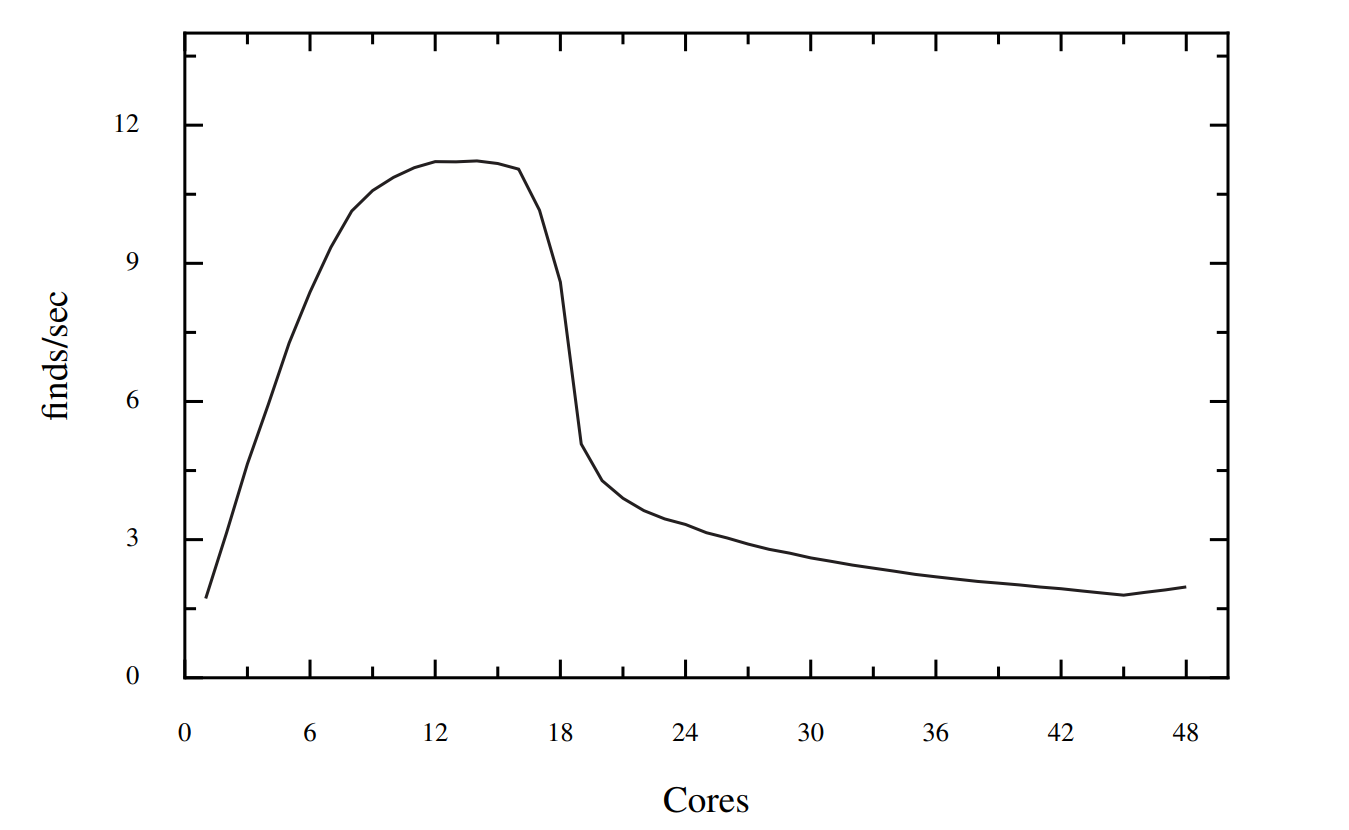
\includegraphics[width=\linewidth]{ticket.png}
	\caption{افت کارایی در استفاده از قفل بلیت}
\end{figure}